\chapter{绪论}
\thispagestyle{others}
\pagestyle{others}
\xiaosi

\section{研究背景及意义}
    随着科技进步和经济发展,人工智能已悄然融入人们的日常生活,智能产品正潜移默化地改变着生活方式、交通出行和娱乐方式。其中,无人驾驶\upcite{levinson2011towards,JGDJ201913001,QCDQ202306002}、机器人\upcite{zhou2022loop,CUXI202211032}以及增强现实和虚拟现实\upcite{carmigniani2011augmented,JSJZ202303043}等领域备受关注。这些技术的出现不仅使人们的生活更加便捷,出行更为高效,同时也丰富了娱乐体验。然而,在机器人和自动驾驶等应用中,环境感知能力是实现高级智能的核心,一个可靠的感知系统对于自动避障和环境识别至关重要。为确保实际应用中的安全性与准确性,优秀的感知系统往往需要集成多种传感器进行多模态数据采集,而激光雷达正是其中的一个关键传感器。激光雷达通过固定频率和角度发射激光,接收返回信号以采集周围环境信息,生成包含三维空间几何信息的点云数据,这一点是二维图像所无法提供的。此外,其采集的数据不受光照变化影响,能够真实还原物体的尺寸和形态,基于这些优势,激光雷达已被广泛应用于各种智能系统中。因此,如何高效利用三维点云数据实现精准感知,已成为当前非常重要的研究课题。
    \begin{figure}[H]
        % \vspace{-0.1cm}
        \centering
        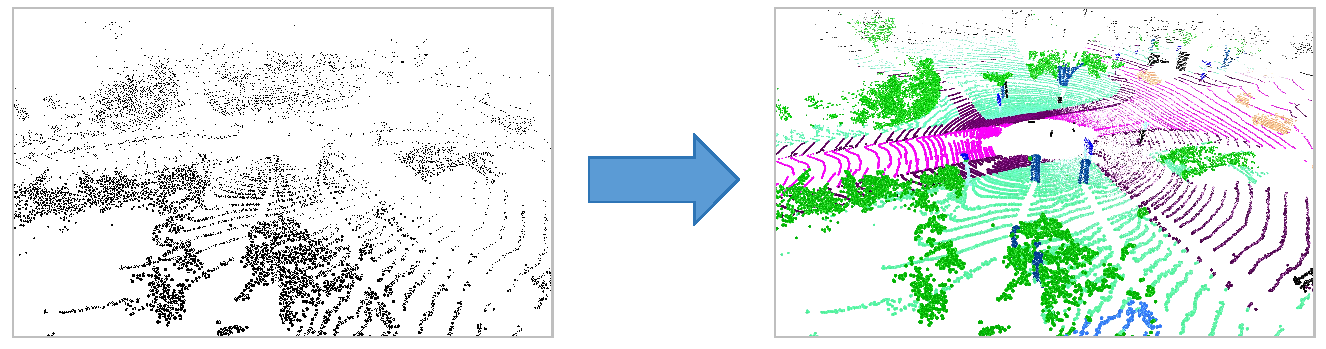
\includegraphics[width = \textwidth]{ljx/figure/1-1.pdf}
        \bicaption[\xiaosi 点云语义分割]{\wuhao 点云语义分割}{\wuhao Point cloud semantic segmentation}
        \label{fig:1-1}
        % \vspace{-0.1cm}
    \end{figure}
    点云语义分割是实现三维场景感知的关键任务\upcite{JGDJ201904002,KXTS202101001,JSGG202001005}。在无人驾驶和机器人领域,通过对周围环境和道路进行语义分割,可以为不同类别的点赋予相应的语义标签,从而将原始点云数据转化为含有语义信息的三维场景数据,如图\ref{fig:1-1}所示。基于此,系统能够依据环境中的语义标签有效区分不同物体,并据此调整导航路径,确保车辆或机器人的正确行进方向。在增强现实中,准确的语义分割则是实现虚拟内容与真实环境无缝融合的前提,只有对真实世界中的物体及其边界进行精确感知和分类,才能将虚拟场景合理地叠加到现实世界中,达到增强现实的效果。尽管点云语义分割的应用价值巨大,早在深度学习兴起之前便已引起学术界广泛关注,但受限于传统机器学习方法在处理大规模点云数据时的效率和性能不足,其研究进展较为缓慢。

    随着深度学习技术的发展,端到端的点云语义分割方法在大规模数据处理和分割精度上均取得了显著提升,大量优秀模型如雨后春笋般涌现,为该领域注入了新的动力。值得注意的是,由于点云数据集根据获取场景的不同又可以分为室内点云数据集\upcite{S3DIS,Scannet}和室外点云数据集\upcite{behley2019semantickitti,caesar2020nuscenes,pan2020semanticposs},它们各具特点。室内数据集密度均匀且规模相对较小,多用于增强现实和机器人等应用;而室外数据集则呈现近密远疏的特性,覆盖的场景更为广阔,通常用于无人驾驶等领域。尽管基于深度学习的算法在这两类数据集上均取得了显著进展,并为实际应用带来了美好前景,但这些算法普遍依赖于逐点标注数据进行全监督训练。然而现实中,一帧点云通常包含十多万个点,一个场景可能包含数千帧点云,而一个完整的数据集则可能涉及十多个不同场景。由于点云本质上是无序的几何数据,其标注工作需要专业人士操作,因此逐点标注不仅复杂而且极为耗时\upcite{behley2019semantickitti}。高昂的标注成本已成为制约这些先进算法落地应用的重要挑战。因此,如何在标注成本与模型性能之间取得平衡,以及如何利用已有数据或仅用少量标注数据训练出高性能的分割模型,成为亟待解决的关键问题。

    域适应作为解决上述问题的重要研究分支,其基本思路是利用已有逐点标注的全监督数据训练预训练模型,再将该模型迁移到未标注的目标域中,同时解决由于场景差异或传感器差异所引起的域偏移问题。常见的域适应方法包括无监督域适应、半监督域适应和主动域适应。无监督域适应虽然不依赖目标域标注,但其效果与全监督方法仍存在较大差距;半监督域适应虽然优于无监督方法,但由于目标域中标注数据通常为随机采样,受域偏移影响较大,其作用未能充分发挥。相比之下,主动域适应通过结合主动学习方法,从目标域中选择对模型迁移最有价值的样本进行标注,既有效缩小域间隙、提升了模型性能又降低了标注成本。
    
    然而,目前基于语义分割的主动域适应研究主要集中在二维图像领域,而在三维点云领域尚缺乏系统性的探索。此外,传统的主动学习方法难以直接应用于域适应场景;同时,由于主动学习选择的样本数量较少,如何充分利用源域和目标域的标注数据,既发挥各自潜力又有效防止域偏移累积和类别不平衡,仍是需要解决的问题。因此,本文的研究以主动学习和域适应为出发点,首先通过大量文献调研,基于域适应的特点寻找适用于三维点云语义分割任务的主动查询策略;随后,深入探索主动标注样本与源域数据的有效融合的主动混合方法,以期获得更加稳固的跨域特征表示。最后,通过大量实验对提出方法进行验证分析。

\section{国内外研究现状}
本文主要研究方向为点云语义分割任务下的主动域适应,因此重点是探索适合点云语义分割域适应任务的主动学习方法,并在此基础上进一步研究适合主动学习的混合(Mixing)方法,因此相关工作涉及到点云语义分割、主动学习、域适应以及Mixing数据增强等相关领域。所以本节将分别对这四个领域中最近几年的相关研究和进展进行分析和总结。
\subsection{基于深度学习的点云语义分割方法}
由于传统机器学习方法难以高效且精确地对大规模点云数据实现逐点分割,基于端到端的深度学习方法因其大批量数据处理能力已成为点云语义分割任务的主流方法。这些方法大致可以分为三类:基于二维投影的点云语义分割方法、基于体素的点云语义分割方法和基于点的点云语义分割方法。

基于二维投影的方法通过不同的投影视角将无序非结构化的点云投影到结构化的二维图像中,投影方法包括鸟瞰图\upcite{aksoy2020salsanet},球形\upcite{cortinhal2020salsanext,RangeNet++,wu2018squeezeseg,wu2019squeezesegv2,xu2020squeezesegv3},多视角\upcite{boulch2017unstructured,kundu2020virtual}等。然后利用更加成熟稳定的二维卷积网络去对这些点云图片进行特征提取和语义分割,并将分割后的结果映射回点云中。此类方法的核心思想是模态转变,将点云从三维转变为图像,然后就可以利用二维卷积网络处理。但是其不足也非常的明显,二维和三维模态差异导致其表征信息的方式也有所不同,模态的转换导致三维几何信息被破坏,进而造成信息的丢失。因此,完全基于投影的方法在随后的研究中,逐渐被人遗忘,研究者们转而开始寻找更加有效的点云语义分割的处理方式。有研究者认为图像模态下的点云可以提取不同于三维模态下的特征,为了充分利用图像提取到的信息,提出了混合点云三维特征和二维特征的多模态方法,这种方法将两者的处理结果相结合,形成了优势互补\upcite{robert2022learning},并成功取得非常可观的分割效果。

基于体素的方法首先将三维点云数据转换为体素网格,即将原本离散且稀疏的点云数据规整成规则的三维格状结构,接着利用稀疏卷积技术在该结构上进行特征提取和表示学习,从而获得较为紧凑且具有表达能力的点云特征。这种方法在处理大规模室外场景时表现出较高的效率,因为规则化的体素结构便于卷积操作的实现,并可显著降低计算复杂度。然而,体素化过程中由于数据离散化的固有属性,往往会导致细节信息的损失,尤其是在高分辨率特征提取方面存在一定局限。这些方法中有一些是比较优秀且至今仍被作为基础框架研究的。MinkowskiNet\upcite{MinkowskiNet}提出了一种高可用到的稀疏卷积方法,并构建了一个专门用于稀疏张量的自动微分库。基于这一方法与工具,构建出一种四维卷积神经网络,用于时空感知任务,其设计能够同时捕捉空间与时间维度的信息,实现更为精准的特征提取。而之后提出的一些稀疏卷积方法\upcite{graham20183d,tang2020searching}则是对许多无意义的计算消耗进行了改进,进一步提高了计算效率。最新的基于体素的方法OA-CNNs\upcite{peng2024oa}则提出了一种全自适应三维卷积神经网络,该网络由动态感受野和自适应关系映射组成:空间动态感受野能够根据输入数据的分布灵活调整感受区域;自适应关系卷积,用于捕捉并建模局部特征之间的复杂关联。因此其在一定程度上展现了超越Transformer架构的潜能。由于点到体素的转换,一定程度上缓解了计算消耗,因此这些方法更适用于大规模的室外点云场景处理。

基于点的方法直接将点云输入到分割网络而不进行任何处理。在提出PointNet\upcite{qi2017pointnet}架构之前,三维点云特征的提取都是手动完成的。PointNet是第一个能够直接使用三维点云提取深度学习特征的架构。其通过提取点云特征中的最大值来处理点云的无序特性,然而这也会导致其无法利用点云中的局部结构信息,无法运用到大规模数据集上。而它的改进版本PointNet++\upcite{qi2017pointnet++}的主要贡献在于提出了分层结构,使用多个抽象层进行特征提取, 从而实现邻域局部特征和全局特征的提取。受PointNet的影响和启发,更多的基于点的方法\upcite{thomas2019kpconv,li2018pointcnn}被提出。其中,KPCov\upcite{thomas2019kpconv}提出了一种新型点卷积算法,其利用一组核点来确定卷积核权重的作用区域,从而在保留点云完整几何信息的同时克服了传统点卷积的局限性。该方法借鉴了图像卷积的思想,但通过灵活定义核点的数量和位置,实现了对局部特征的高效提取,并以相关函数确定其影响范围。采用半径邻域和规则下采样策略,有效应对了非均匀采样问题,从而在大规模点云场景下保持较高鲁棒性和计算效率。此后,RandLA-Net\upcite{hu2020randla}引入了一个局部特征聚合模块,有效地保留来自大范围邻域的有用特征,并在其方法中使用随机采样,以显著减少内存占用和计算成本。SCF-Net\upcite{fan2021scf}提出了一个可学习的模块(Spatial Contextual Features, SCF),由三个部分组成:局部极坐标表示模块(Local Polar Representation, LPR)、双重距离注意力池化模块(Dual-Distance Attentive Pooling, DDAP)和全局上下文特征模块(Global Contextual Feature, GCF)。LPR模块在极坐标系中构建z轴旋转不变的表示,以捕捉每个3D点的局部上下文。DDAP模块通过利用几何距离和特征距离学习的权重,整合邻域点的表示,学习有效的局部特征。GCF模块利用邻域的位置和体积比,学习每个3D点的全局上下文。SCF模块可以嵌入到各种网络架构中用于点云分割,但其网络结构比较复杂。BBAF-Net\upcite{qiu2021semantic}通过引入密集区域来增强局部上下文解决相邻点的模糊性,同时自适应地融合多分辨率特征,以获取关于点云的全面知识。

随着注意力机制下大模型的爆火,Transformer\upcite{zhao2021point}首次将注意力机应用到点云语义分割任务中。随后的一些工作也将其加入到自己的方法中\upcite{JSJF202203012,GXJM202207010},虽然注意力机制完美适配了点云的无序特性,然而这些方法大多需要更多的计算时间。TransformerV3\upcite{wu2024point}探索了一种新的序列化邻域机制,将点云按照特定模式组织起来。并采用简化方法取代了更复杂的注意力区域交互机制,从而更适用于序列化点云处理。同时消除了对相对位置编码的依赖,并采用了一种更简单的前置稀疏卷积层进行特征提取,从而提高计算效率。基于点的方法能够完整保留点云中每个点的原始几何信息和局部特征,这一优势使其在三维语义分割任务中展现出独特的潜能。当前虽已有不少相关方法取得了显著进展,但在深层次特征利用以及复杂场景的细粒度信息捕捉方面,仍存在大量未被充分挖掘的可能性。随着计算机视觉与深度学习技术的不断演进,未来在这一领域内定将涌现出更多创新方法,为三维数据的高效处理和精准理解提供更加完善的解决方案。

虽然上述算法都在基于深度学习的点云语义分割任务中取得了优异的结果,但是这些方法仍然需要基于全标注的数据进行训练才能实现最佳的效果,而对于点云语义分割任务来说,逐点标注是极其复杂的一项工程。如何平衡性能与标注是一个非常重要的研究方向,主动域适应是其中一个方法, 也正是本文的研究目的所在。

\subsection{视觉语义分割中的主动学习方法}
随着深度学习的发展,模型高性能与数据标注困难以及无标注但性能低的问题也逐渐显现,因此一些研究者开始将目光转向能够平衡性能与标注花费的主动学习上来。在视觉语义分割任务中,根据其筛选的基本单元的不同,大致可以将其分为基于样本的主动学习方法, 基于区域的主动学习方法和基于最小语义单元的主动学习方法。
\subsubsection{基于样本的主动学习方法}
在主动学习的早期阶段,研究者们主要采用以样本作为基本查询单位的方法。这一策略源于主动学习最初在视觉分类任务中的应用,而在这些任务中,数据通常是以单个样本为单位进行划分和标注的。因此,许多针对语义分割任务的早期方法也从分类任务中获得了启发,采用在每一轮数据选择中筛选出信息量丰富的样本并进行逐点或者逐像素的标注。

Tan等人\upcite{tan2019batch}的研究重点在于充分挖掘类别的边缘信息。他们提出了一种方法,首先借助边缘检测器提取图像中的边缘特征,然后将这些边缘信息与利用KL散度评估的不确定性及数据代表性相融合,以实现主动样本选择。该方法将传统的人工设计理念与任务的实际需求紧密结合,取得了显著成效。Sinha等人\upcite{sinha2019variational}出了一种新的池化主动学习算法,该算法基于变分自编码器和对抗网络,通过隐式学习采样机制来选择最具代表性的查询样本进行标注,从而提高模型性能并降低标注成本。Zhang等人\upcite{zhang2020state}提出了一种状态重新标记对抗性主动学习模型,模型充分利用标注信息和状态信息,用于推导出对于当前模型来说信息最丰富的未标记样本。其设计了一种在线不确定性指示器,重新标记未标记数据的状态,赋予其不同的重要性,同时构建了一个无监督的图像重建器和一个监督的目标学习器,生成图像的统一表示,迭代嵌入标注信息。最后结合所提出的k-center方法的初始采样算法,使后续采样更加高效。但这些方法通常以全局不确定性或多样性为准则筛选样本,忽略了语义分割任务中不同区域的内在难度差异,导致标注资源浪费且模型在困难区域表现不足。为了解决这个问题, Xie等人\upcite{xie2020deal}提出了难度感知的主动学习方法(Difficulty-awarE Active Learning, DEAL)。该方法通过引入语义难度分支和设计像素级概率注意力模块动态学习不同语义区域的难度分数,并利用分割误差作为监督信号,使模型准确捕捉那些易混淆或低置信度的像素区域,从而将主动学习的焦点从整体信息量转向局部难度感知。为了解决困难区域样本稀缺的问题,该方法进一步提出了一种双阶段样本获取策略,基于语义难度分数筛选出包含高难度区域的图像,并结合区域不确定性和多样性对像素级标注进行优先级排序,实现了从图像级粗筛选到像素级细粒度标注的渐进式优化。Huang等人\upcite{huang2021semi}利用一种新颖的无标签数据采样策略,结合半监督训练方案进行数据注释,从而利用无标签数据提升任务模型的性能。

基于样本的主动学习方法虽然能够降低标注成本,但在视觉语义分割任务中也存在一些不足。由于一幅图像往往包含多个类别,而各类别的区域大小和分布差异明显,所选样本中的大部分信息可能仅集中在部分类别,其他区域则容易成为噪声。而且标注过程中常见的类别不平衡问题可能导致模型在训练时偏重于主流类别,从而忽略细节部分。此外,语义分割需要对每个像素或者点进行精细判断,单纯依赖样本级的选择往往难以捕捉到局部的复杂信息,这在处理复杂语义区域时尤为明显。

\subsubsection{基于区域的主动学习方法}
在语义分割任务中,基于样本的主动学习方法问题逐渐显现,一些研究者开始寻找缓解问题的方法。由于不同的区域对样本的影响程度不同,因此基于区域的主动学习方法被提出,这种方法将样本划分为不同的区域并作为查询和标注的基本单元。Qiao等人\upcite{qiao2022cpral}提出了一种基于区域的主动学习方法框架(Collaborative Panoptic-Regional Active Learning, CRPAL),通过结合全景和区域信息选择策略,有效平衡了标注工作量和模型性能。该框架引入了区域高斯注意力模块来缓解类别不平衡问题,并通过上下文标签扩展模块区域标注,进一步提高了标注效率。但是这种方法的划分是基于规则区域的,即将图像规则划分为同等大小的区域,然而语义类别在图像上的分布往往是不规则的,因此规则区域虽然有效降低了标注成本,却依然存在区域内类别不平衡或者分布不均匀的问题,导致少量的语义类别学习困难。Siddiqui等人\upcite{siddiqui2020viewal}提出了一种基于不规则区域面向深度图像的主动学习方法。其设计了一种基于KL散度的最优视角选择标准,用于衡量预测概率分布在不同视角之间的变化。通过分析预测在不同视角下的不一致性来估计模型的不确定性,并将其定义为视角熵。最后将视角熵与超像素区域选择相结合,使得模型能够高效地筛选出高价值的样本区域。针对普通图像,Cai等人\upcite{cai2021revisiting}也提出了一种类别平衡的采样策略,以提升超像素方法的性能,该策略能够优先选择来自低占比类别的高信息量样本。方法通过计算每个区域的最小边际不确定性,再依据每个区域主导类别所占比例对不确定性进行调整,从而获得更精准的不确定性度量。同时该文章也通过一系列的实验证明了不规则超像素在降低标注成本方面优于规则化的区域。

而在三维点云语义分割的主动学习方法中,区域的划分根据点云的非结构化几何特征而呈现出多样性。Lin等人\upcite{lin2020active}提出了一种主动增量学习框架,通过迭代地选择高信息量样本,逐步丰富模型知识,从而有效降低标注需求。该方法将点云数据被划分为多个小块,并分为已标注和未标注两组。已标注的小块用于训练,在初始迭代中,网络从零开始训练。在后续迭代中,采用微调策略,使模型在已有知识的基础上不断扩展。每轮训练完成后,网络会根据点熵、分割熵和互信息评估未标注点云小块的信息量,并选择最具信息价值的小块进行标注。Wang等人\upcite{wang2023one}提出了一种结合准场景级弱标签的主动弱监督框架,用具有固定半径的球形子点云作为查询单位,每个子点云类别仅需一个点级标签,通过主动策略识别并选择最具信息量的子点云进行标注,从而同时兼顾场景级和点级语义信息。Xie等人\upcite{Annotator}则是将点云划分到同等大小的体素网格中,然后对网格中的点的类别进行预测,计算其内部类别点的熵程度,值越高说明体素网格中包含的不同的类别的点越多,体素网格中的点类别分布越平衡,包含信息越丰富。除了上述规则的方式以外,其实更多的则是通过不规则区域即超点的形式进行的区域划分。

Shao等人\upcite{shao2022active}提出了一种结合类平衡不确定性和多样性的采样策略。该策略引入加权超点不确定性估计,根据超点中类别数量的多少赋予这些不同类别点不同的权重,以更准确地衡量超点的不确定性。同时,通过空间结构多样性推理机制,构建出超点图和图聚合操作,将超点特征投影到多样性空间中,利用最远点采样选择最具代表性的超点进行标注。Hu等人\upcite{hu2022lidal}提出了一种新颖的基于视角一致性的不确定性度量方法,以利用帧间约束信息。该方法基于连续 LiDAR帧中预测分数函数的方差,设计了新的帧间散度和熵公式,对于一个未标注目标,如果其预测标签在不同帧之间存在较大差异,便认为模型预测不可靠,并选择这些最具不确定性的区域进行人工标注。与Hu利用时序帧间一致性的思路不同,Liu等人\upcite{liu2024active}提出了一种基于多版本预测一致性的主动学习策略,通过数据增强构建输入点云的多个变体,以评估模型预测的稳定性。针对每个点在不同增强版本中的预测结果,计算其对应最高置信度类别的概率分布标准差作为不确定性度量,为缺乏连续帧数据的场景下提供了更灵活的标注策略。而Wei等人\upcite{wei2024basal}则提出了一种基于尺寸平衡的主动学习方法,旨在解决点云语义分割中的类别不平衡与冷启动问题。该方法主要通过物体尺寸特征间接平衡类别分布,将不同尺寸的物体聚类为同一类别,在选择的时候优先选择各类别分区中信息量最大的簇进行标注。基于区域的方法由于在标注和性能上都有所突破,因此仍是语义分割任务中比较主流的方法。
\subsubsection{基于最小语义单元的主动学习方法}
语义分割任务中基于区域的主动学习方法显著优于基于样本主动学习的方法。为进一步优化标注效率,部分学者提出将选择粒度细化至最小语义单元,旨在通过精准标注关键局部区域,实现以更低成本的更高表现。在二维图像中,最小的语义单元是像素,因此在面向图像的基于最小语义单元的主动学习方法中,都是以像素为基本选择和标注单位。Shin等人\upcite{shin2021all}提出了第一个基于像素的主动学习框架,该方法将基于边界的不确定性策略运用到了不同的图片像素间,并比较不同像素间的差异作为衡量指标。该方法证明了仅在少量像素点上提供标注的情况下,深度神经网络能否依然取得良好表现,并证明在语义单元层面的标注,模型仍然能够有效学习语义信息。Rückin等人\upcite{ruckin2024semi}则是进一步将基于像素的主动学习方法与半监督学习相结合,并运用到了实际场景中。这一举措从实际运用层面证明了基于像素的主动学习标注的有效性和和高效性。而在三维点云语义分割中,最小语义单元是点。Xu等人\upcite{xu2023hierarchical}提出了第一个基于点的主动学习方法,该方通过加权计算每个点与不同下采样层次的周围领域信息的熵值总和,然后选择出不确定性排名靠前的点,同时通过一种特征距离抑制的方法来过滤空间距离相近且类别相似的冗余点。该方法不仅提高了模型性能,也大大增加了有效标注率。以上这些主动学习方法不仅显著降低了所需的标注比例,还能在保持模型性能达到全监督水平约90\%的前提下,大幅降低人力成本。但是,传统的主动学习方法主要适用于单一数据集,对于存在显著域间差异的域适应任务则难以直接应用。
\subsection{视觉语义分割域自适应方法}
殊途同归,与主动学习不同的是域自适应方法则通过模型迁移的方式来解决目标域数据需要大量标注的问题。其核心思想是将在有标注的数据上训练好的模型迁移到无标注的目标域上去,并解决因域偏差而导致的模型性能下降问题。基于视觉语义分割的域自适应方法大致可以分为三类:无监督域自适应方法、半监督域自适应方法以及主动域自适应方法。
\subsubsection{无监督域适应}
目前,在三维点云领域,研究者们更多地关注基于无监督的域自适应方法。当聚焦于点云语义分割任务时,根据跨域数据集的差异,这些方法又可以分为两类:真实到真实的场景,以及合成到真实的场景。真实到真实的无监督域自适应方法,通过使用LiDAR传感器捕获的真实场景数据进行深度网络训练,随后在不同LiDAR传感器捕获的未知场景中进行测试。在这种情况下,Yi等人\upcite{yi2021complete}将域适应形式化为3D表面补全任务,该方法通过设计并训练一个上采样网络,将雷达线束补全到统一的64线,然后再将补全后的数据输入到分割模型进行分割。而Langer等人\upcite{langer2020domain}则通过射线投射将目标域的传感器模式转移到源域。在合成到真实的域自适应中,源数据通过模拟LiDAR传感器获得非真实场景的合成数据,而目标数据则由真实LiDAR传感器采集。在这种情况下,域偏移是由于采样噪声、环境结构和类别分布的差异引起的。Wu等人\upcite{wu2018squeezeseg}认为注意力模型可以用于聚合上下文信息,并且可以采用逐步域校准的测地线相关对齐来改善域自适应。在后续的文章中,Wu等人\upcite{wu2019squeezesegv2}则是通过生成对抗网络在合成数据上模拟真实的点云噪声。

类似地,Xiao等人\upcite{xiao2022transfer}将域偏移分解为外观差异和稀疏度差异,然后应用生成网络来减轻每个差异。Saltori等人\upcite{saltori2022cosmix}则是通过对源域和目标域分别进行语义选择而后进行混合再放入到师生模型中进行训练,从而提高模型的性能。Ding等人\upcite{ding2022doda}提出了一个可以运用在室内数据集上的方法,其注意到了长尾类问题,设计了一个长尾类别注意机制,把已经打好伪标签的目标域长尾类别数据和源域进行混合后一同放入模型中训练。Bian等人\upcite{bian2022unsupervised}提出了一个基于图的框架来探索两个域之间的局部级特征对齐,在两个域上动态构建局部特征图,并利用源域的图建立记忆库,使用最优传输来生成图匹配对,最后基于图的局部特征损失来调整两个域之间的特征分布。Jiang等人\upcite{jiang2021lidarnet}设计了一个可以提取领域共享特征和领域私有特征的模型,然后利用GatedSCNN网络使领域共享特征提取器能够在领域共享特征中保留边界信息,并利用学习到的边界来完善分割结果。然而这些方法与在全监督下测得的目标数据集的性能上界仍存在很大的差异。
\subsubsection{半监督域适应}
为了解决无监督域适应与全监督性能差距过大问题,一些学者提出了基于半监督以及弱监督的域适应方法,但是这些方法目前在三维点云中出现的并不多,尤其是在三维语义分割领域中。Jaritz等人\upcite{jaritz2022cross}提出了第一篇点云语义分割领域的半监督域自适应。其使用跨模态的方式进行学习,利用点云几何先验信息以及图像的纹理颜色信息,并取二者的优点进行互补,使得提取的特征更加鲁棒,其具体实现是设计了一个双流、双头架构,一端是图像输入,一端是点云输入,在三维语义分割任务中对图像和点云模态应用了跨模态损失。跨模态损失包括应用于两种模态预测之间的KL散度,从而加强一致性。Chen等人\upcite{chen2021semi}提出了双层面域混合架构,从样本和区域层面混合两个域,生成两个老师模型,并通过这两个老师模型蒸馏知识给一个学生模型,使得学生模型更加强大,而其生成的伪标签将继续用于下一次双域混合中训练老师模型。Saito等人\upcite{saito2019semi}提出了一个由特征编码网络组成模型,使用一个分类层,用来计算特征与一组估计类别代表的相似性。通过交替地最大化未标记目标数据相对于分类器的条件熵和最小化其相对于特征编码器的条件熵来实现自适应。

Yu等人\upcite{yu2023semi}则是从数据的角度来看问题,认为原始源标签可能存在噪声,因此将域自适应作为一个噪声标签学习问题,并利用具有伪中心的质子集的预测来修正源标签。Saltori等人\upcite{saltori2023compositional}设计了一种双分支对称网络架构,能够同时处理来自源域和目标域的点云,并通过跨域语义混合来减少域间分布差异。该方法基于教师-学生框架,在源域和目标域之间混合点云片段,然后利用源标签和目标伪标签进行监督,同时结合少量人工标注数据进一步提升性能。尽管在少量真实标注的支持下,半监督域自适应方法相较于无监督方法已经取得了显著的性能提升,但与目标域下全监督的结果仍存在一定差距。同时,半监督方法中所采用的标注往往具有较大的随机性,无法确保每个标注点都能有效地促进模型性能提升,这在一定程度上暴露了标注效率的问题。
\subsubsection{主动域适应}
基于半监督和弱监督的方法在一定程度上提升了模型性能,但其标注点的选取往往是随机进行的,这使得数据利用效率和标注效果存在一定局限。为实现更高效的标注并充分挖掘数据的潜在价值,部分学者开始探索将主动学习与域适应技术相融合,通过主动学习策略在目标域中主动选取那些信息量大、价值高的点,而非被动地随机标注低价值数据,同时利用域适应技术最大化这些数据的效用。

然而,传统主动学习策略通常依赖于模型对数据的筛选,而在域适应场景中,模型往往基于源域数据进行训练,由于存在域间隙,这种筛选过程可能导致所选标注点失效,最终引发无效标注的问题。早期的主动域适应研究提出通过利用对抗训练的领域判别器来衡量每个目标实例的不确定性和域特性。不同于之前的方法,CLUE\upcite{CLUE}则提出了一种熵加权聚类算法,用于查询目标域中不确定和多样化的样本。而SDM\upcite{SDM}被提出来优化边际损失函数,以探索与源领域中潜在硬样本相似的目标实例。然而,现有的主动域适应方法大多刻意设计手工制作的查询函数来评估样本的注释值,并对所有目标数据一视同仁地采用相同的适应策略。这种僵化的标准使它们很容易过度适应某些领域的适应情况,从而限制了主动域适应方法的泛化。

一些具有创新性的主动域适应方法,类似Huang等人\upcite{Divide}采取了分而自治的思想,把目标域上的数据分为4类,分别对这类数据进行不同的定制学习,但是这个方法是用在分类任务上的对于语义分割来说难以直接利用。Wang等人\upcite{HPML}发现满足邻近混沌区域、个体差异和来源不相似属性的样本是信息量最大的样本,并将其定义为最小快乐点,并设计了最小快乐点学习方法(Minimum Happy Point Learning, MHPL)以很好地探索和利用最小快乐点,有效提高模型性能。Annotator\upcite{Annotator}是首个将主动域适应方法应用于点云语义分割任务的方案。该方法将点划分至更大的体素块中,并采用专门设计的体素混淆度选择策略,在有限预算下实现了高效的样本选择与性能优化。然而,其主动学习策略并非专门为域适应场景设计,类似于传统主动学习方法,仍忽略了域差异可能导致所选样本在目标域上无法实现最佳提升的问题。

\subsection{视觉语义分割中的混合方法}
混合(Mixing)方法在深度学习中,一直被作为一种数据增强的方式进行使用。其核心思想是通过混合不同的样本或特征来增强模型的泛化能力和鲁棒性,然而不同的任务和模态下的数据其Mixing的方式也有所不同。
2018年,Zhang等人\upcite{zhang2017mixup}首次提出mixup方法,用于超越经验风险最小化。这是第一篇关于Mixing的文章,其通过线性插值的方式将训练样本及其对应的标签进行凸组合,将组合后的数据用以训练模型,从而正则化神经网络,使其在训练样本之间表现出更简单的线性行为。该方法被用于分类任务上,并显著提高了模型的泛化能力,其在面对对抗样本和标签噪声时表现出很强的鲁棒性。然而,mixup在图像分类任务中虽然表现优异,但在语义分割这种需要细粒度分类的任务中存在局限性。

为了解决这一问题,CutMix方法\upcite{yun2019cutmix}被提出。该方法通过切割和粘贴图像区域,结合标签的线性插值,不仅保留了mixup的正则化效果,还能够更好地处理局部特征,从而在弱监督目标定位和图像分类任务中取得了更好的性能。随着研究的深入,Mixing方法逐渐被应用到三维点云数据处理领域。Mix3D方法\upcite{nekrasov2021mix3d}首次被提出,并用于3D场景的上下文数据增强。其通过混合两个增强场景,将对象实例隐式地放置在新的上下文中,从而帮助模型减少对场景上下文的依赖,更多地关注局部结构和特征。为了进一步提升模型在不同领域数据上的适应能力,CoSMix方法\upcite{saltori2022cosmix}被提出,用于3D点云分割的领域自适应。该方法通过组合语义信息和几何信息的样本混合策略,有效地平衡了全局上下文和局部几何结构,从而在不同领域数据上取得了更好的性能。随后,LaserMix方法\upcite{kong2023lasermix}被提出,用于半监督的LiDAR语义分割任务。该方法通过混合来自不同LiDAR扫描的激光束,鼓励模型在混合前后做出一致且正确的预测。该方法在多个主流LiDAR分割数据集上展示了其有效性和优越性。
尽管这些Mixing方法在解决特定问题上展现了卓越的性能提升,但目前它们主要与无监督、半监督乃至弱监督策略相结合,而在主动学习领域的应用仍未得到充分探索,而这正是本文关注和研究的重点之一。

\section{论文研究主要内容}
\begin{figure}[H]
    % \vspace{-0.1cm}
    \centering
    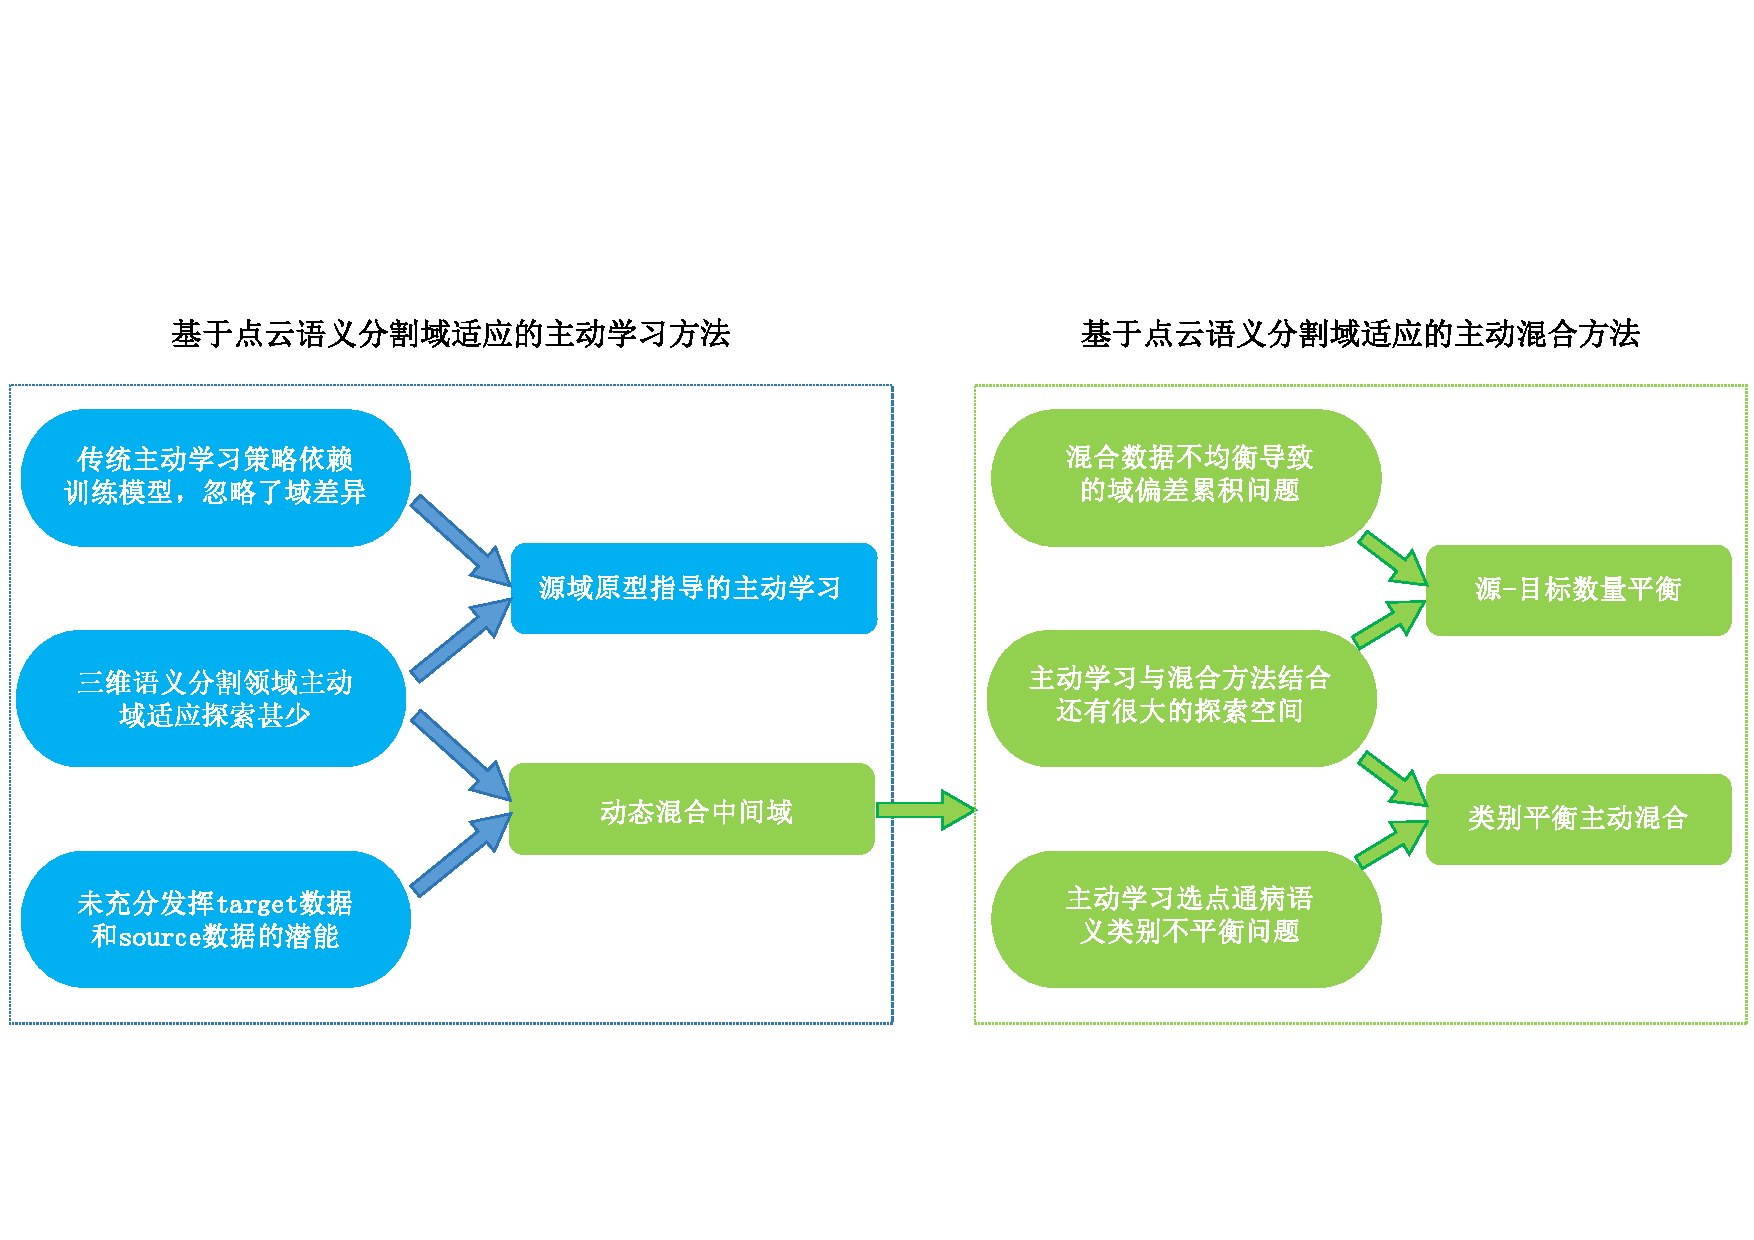
\includegraphics[width = \textwidth]{ljx/figure/1-2.pdf}
    \bicaption[\xiaosi 主要研究内容概要]{\wuhao 主要研究内容概要}{\wuhao Overview of main research content}
    \label{fig:1-2}
\end{figure}
\vspace{-1em}
本研究聚焦于三维点云语义主动域适应问题,旨在探索和设计一种主动学习方法,以选择出对模型迁移最具价值的目标样本。同时,为了充分挖掘源域数据和主动标注样本的潜能,本文设计了一种高效的数据混合方法,将两者有机结合,从而进一步提升模型性能。主要研究内容的概要图如图\ref{fig:1-2}所示,其内容如下:

% 1)大量查阅相关领域文献,对基于深度学习的点云语义分割算法、视觉语义分割中的主动学习方法以及域自适应技术的最新进展及存在问题进行了系统梳理。通过总结上述研究成果,本文阐明了现有方法的优势与不足,并探讨了可改进的方向,为新方法的提出提供了坚实的理论基础。

1)提出了基于点云语义分割域适应的主动学习方法。该方法由三个模块构成:源域原型构建模块、源域原型指导的数据选择模块和动态混合中间域构建模块。首先通过动态构建源域原型来代表源域类别质心,并在每一轮主动学习阶段实时更新原型,在进行目标域候选点筛选时,计算每个目标域中未标注的点与每个源域类别原型的相似度,通过最优-次优差异算法获取归一化后的类别概率的差值得到域差异性评分,同时结合不确定性评分得到最终候选评分,升序排列后选取前 k 个同时兼备高不确定性和高域差异性的目标点。此外,该方法首次将主动学习方法与Mixing方法结合,构建包含目标域信息和源域信息的中间域数据,帮助模型学习到更稳定的域不变特征,进一步缩小域间隙。

2)提出了深度结合混合方法与主动学习的主动混合方法。该方法在基于点云语义分割域适应的主动学习框架上进行了深入探索,旨在解决由于数据量问题导致的域偏移累积以及主动学习选点不平衡问题。具体而言,该方法将动态混合中间域构建模块细分为两个模块:源-目标数量平衡模块和类别平衡主动混合模块。在每一轮主动学习过程中,通过动态匹配源域与目标域标注点的数量,确保混合数据中双域信息的均衡融合;同时,类别平衡主动混合模块保证了混合后数据的类别分布相对平衡,从而增强了主动学习与混合方法之间的协同作用。
\section{论文组织结构}
本文一共分为五个章节,各章节安排如下:

第1章为绪论,主要针对点云分割的研究背景、意义以及国内外的现状做详细阐述。首先介绍点云语义分割主动域适应方法的研究背景和研究意义。其次分别介绍了基于深度学习的点云语义分割方法、视觉语义分割相关的主动学习方法和域自适应方法以及视觉语义分割中的Mixing方法。最后简述本文的主要研究内容以及论文的主要组织架构。

第2章为点云语义分割主动域适应相关理论基础,对点云语义分割,主动学习及域自适应等本文研究涉及领域的基础知识做详细阐述。首先介绍了点云表示及点云语义分割模型基础,并介绍了点云语义分割中的常用评价指标;接着介绍了主动学习的相关基础概念和流程;随后又介绍了域自适应的基础概念和常用域对齐方法;最后对跨域点云语义分割任务中常用的主流公开数据集进行了介绍。

第3章提出基于点云语义分割域适应的主动学习方法。首先介绍了该方法的研究动机和贡献,接着详细的阐述了提出的方法框架和基于原型指导的学习方法,包括动态源域原型构建模块、原型指导的数据选择模块和动态中间域构建模块,最后在合成到真实以及真实到真实
% 最后在合成到真实(SynLiDAR$\to$SemanticPOSS、SynLiDAR$\to$SemanticKITTI)以及真实到真实(SemanticKITTI$\to$nuScenes、nuScenes$\to$SemanticKITTI)
的跨域场景下进行了大量实验验证以及可视化分析证明该方法的有效性。

第4章提出基于点云语义分割域适应的主动混合方法,该方法是基于第3章提出的点云语义分割域适应的主动学习框架上进行主动混合方法的改进。同样首先介绍了该方法的研究动机和研究贡献,接着详细介绍了方法中的主要模块,包括源-目标数量平衡方法和类别平衡主动混合方法。最后在合成到真实以及真实到真实的两个跨域场景、四个跨域数据集下进行了大量实验验证以及可视化分析证明该方法的有效性。

第5章为总结和展望。此章节对全文研究内容进行了全面总结和深入分析,总结了本文在三维点云语义分割主动域自适应中的相关问题、研究内容以及实验结果。最后基于文章总结,对点云语义分割主动域适应任务未来的研究方向提出了展望。

\clearpage